% !TeX root = ../handout.tex

\section{Data Spaces und Data Ecosystems}

% Lieferketten -- IOIS
Daten sind für nahezu alle Geschäftsprozesse notwendig, wie bspw. der Koordinierung und Optimierung von Lieferketten.
\emph{Inter-Organisational Information Systems} (IOIS) (vgl. \autoref{fig:data-sharing-iois-di-ds} links) beschreiben bilaterale Beziehungen, wie bspw. Lieferketten, bei denen individuelle Systeme für eine tiefe Integration und automatisiertem Data Sharing verbunden werden.
Dabei werden Daten für einen bestimmten Zweck geteilt, wie bspw. dem Entgegenwirken schädlicher Effekte in Lieferketten und der Steigerung von Effizienz.
Aufgrund von mangelndem Vertrauen besteht die Angst vor Datenmissbrauch oder unberechtigter Weitergabe von Daten, wie bspw. Betriebsgeheimnissen, weshalb streng formalisierte Nutzungsrichtlinien notwendig sind.
Keine Daten zu teilen würde jedoch zu ineffizienten Lieferketten und somit wirtschaftlichem Verlust führen, was keine Option für Unternehmen ist.
Eine Skalierung solcher Beziehungen bringt jedoch Herausforderungen mit sich, wie bspw. Kontrollverlust oder unberechtigte Datenweitergabe~\cite{mollerIndustrialDataEcosystems2024}.

\begin{figure}
    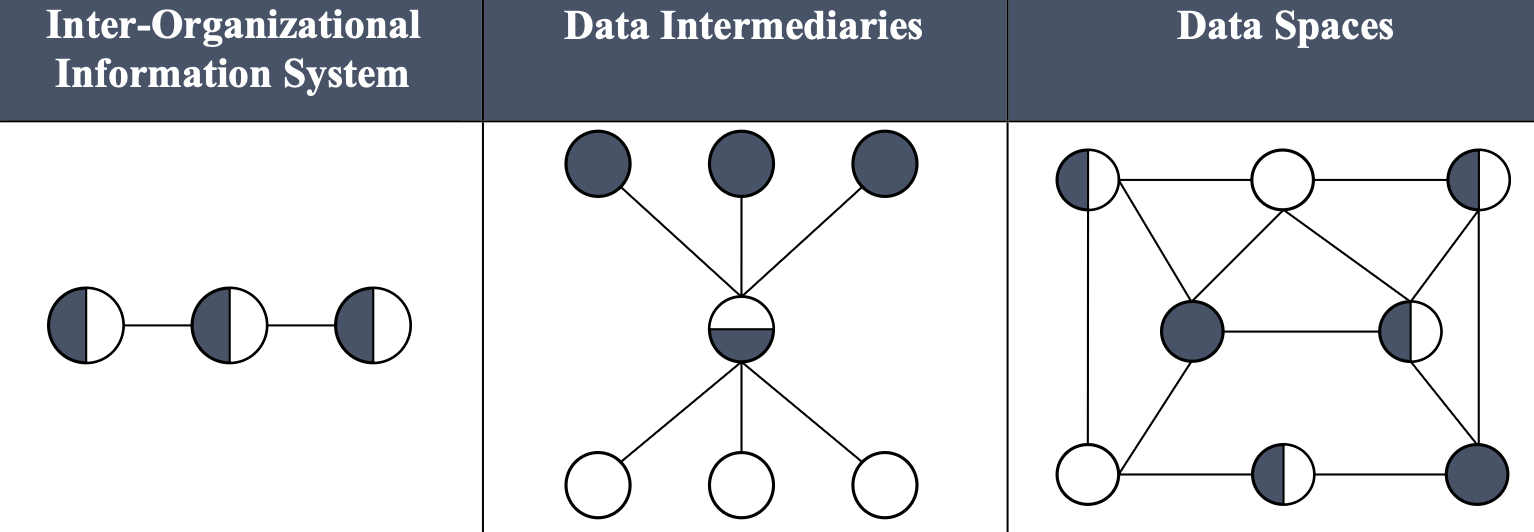
\includegraphics[width=\textwidth]{./assets/moller_iois_di_ds.png}
    \caption{Data Sharing in IOIS, Industrial Data Ecosystems mit Data Intermediaries, sowie Data Spaces~\cite{mollerIndustrialDataEcosystems2024}}
    \label{fig:data-sharing-iois-di-ds}
    % TODO: Bild ersetzen
\end{figure}

% Industrial Data Ecosystems -- Data Intermediaries
Daher ist eine alternative Sicht auf zwischen"=betriebliches Data Sharing entstanden: \emph{Industrial Data Ecosystems} (vgl. \autoref{fig:data-sharing-iois-di-ds} mittig).
% TODO: wie generieren diese Vertrauen?
Diese entwickeln sich dynamisch um einen geteilten Zweck und erhalten ein Gleichgewicht zwischen erhaltenem und gegebenem Aufwand.
Daten sind somit nicht mehr nur Mittel zum Zweck, sondern eine strategische Ressource, um neue Geschäfte zu ermöglichen und Prozesse zu optimieren.
Dies geschieht durch \emph{multilaterale} Akteure, welche miteinander interagieren und kooperieren.
Jeder Akteur kann dabei zum Data Sharing beitragen, in dem Daten verwendet (\emph{Data User}) oder bereitgestellt (\emph{Data Provider}) werden.
\emph{Data Intermediaries} agieren als zentraler Akteur, welche zwischen Data User und Provider vermitteln können, wodurch ein  multilaterales Netzwerk für einen offenen und dynamischen Datenaustausch geschaffen werden kann.
Sie aggregieren, verarbeiten und verteilen relevante Daten, um deren Wert zu maximieren.
Dadurch können Netzwerkeffekte entstehen und Innovation gefördert werden~\cite{mollerIndustrialDataEcosystems2024}.

% Data Spaces
\emph{Data Spaces} vereinen die Konzepte von IOIS und Data Intermediaries.
Aufgrund der dezentralen Speicherung von Daten bei Data Providern werden \emph{Data Space Connectors} verwendet, um einen bilateralen Datenaustausch zu ermöglichen (vgl. IOIS).
Dieser erfolgt erst nach einer erfolgreichen Verhandlung der Rahmenbedingungen.
Ähnlich wie Data Intermediaries bringen Data Spaces verschiedene Data Provider und User zusammen, um Netzwerkeffekte zu schaffen.
Die Kontrolle über den Zugriff und Verwendung von Daten liegt stets beim jeweiligen Data Provider.
Betriebliche Barrieren werden überwunden, in dem Datensouveränität technisch garantiert wird.
Dadurch wird ein geteilter Raum für Akteure geschaffen, in dem ein vertrauenswürdiger Datenaustausch statt finden kann, wodurch zwischenbetriebliche Optimierung und Innovation gefördert werden kann~\cite{mollerIndustrialDataEcosystems2024}.

% Eigenschaften von DS
Data Spaces sind verteilt \emph{by Design} wodurch keine physikalische Datenintegration notwendig ist.
Die Daten bleiben bei der Quelle (Data Provider), wobei der Zugang nur gewährt wird, wenn dieser notwendig ist.
Aus der verteilten Architektur folgt, dass Daten an verschiedenen Orten koexistieren können (Datenredundanz).
Außerdem ist kein einheitliches Daten"=Schema notwendig, da die Datenintegration auf semantischer Ebene, bspw. durch einheitliche \emph{Vocabularies} stattfindet.
Weiterhin können Data Spaces verschachtelt oder überlappend sein, in dem Data Provider oder User mitglieder verschiedener Data Spaces sind.
Somit können \emph{Data Ecosystems} um einen oder mehrere föderierte Data Spaces entstehen, welche über Schnittstellen technisch integriert werden, wodurch gemeinsame Ziele der Akteure realisiert werden können.
Um große Daten"=Silos zu verhindern, sind überlappende Data Ecosystems mit verbunden Data Spaces anzustreben.

% Data Ecosystem Parties
Data Spaces erlauben flexible betriebliche Strukturen, welche einer bestimmten Menge an Akteuren Zugriff auf den sicheren, vertrauenswürdigen Data Space erlauben, welcher in größere \emph{Data Ecosystems} eingebettet werden kann.
Akteure aus einem Ökosystem können ebenfalls zum Datenaustausch beitragen ohne selbst Teil des Data Spaces zu sein.
Im Gegensatz zu \emph{Data Space Members}, welche direkt technisch in den jeweiligen Data Space eingebunden sind, greifen sog. \emph{Data Ecosystem Parties} nur indirekt über Data Space Connectors auf den Data Space zu. % (vgl. \autoref{fig:data-ecosystem})
Diese dienen als Schnittstelle zwischen Data Space Members und dem Data Space an sich.
Um rechtliche Anforderungen, bilaterale oder multilaterale Regeln zu garantieren, können Governance"=Maßnahmen auf allen Abstraktionsebenen -- d.h. auf der Ebene von Data Ecosystems, Data Spaces oder Use Cases -- etabliert werden~\cite{mollerIndustrialDataEcosystems2024}.

% \begin{figure}
%     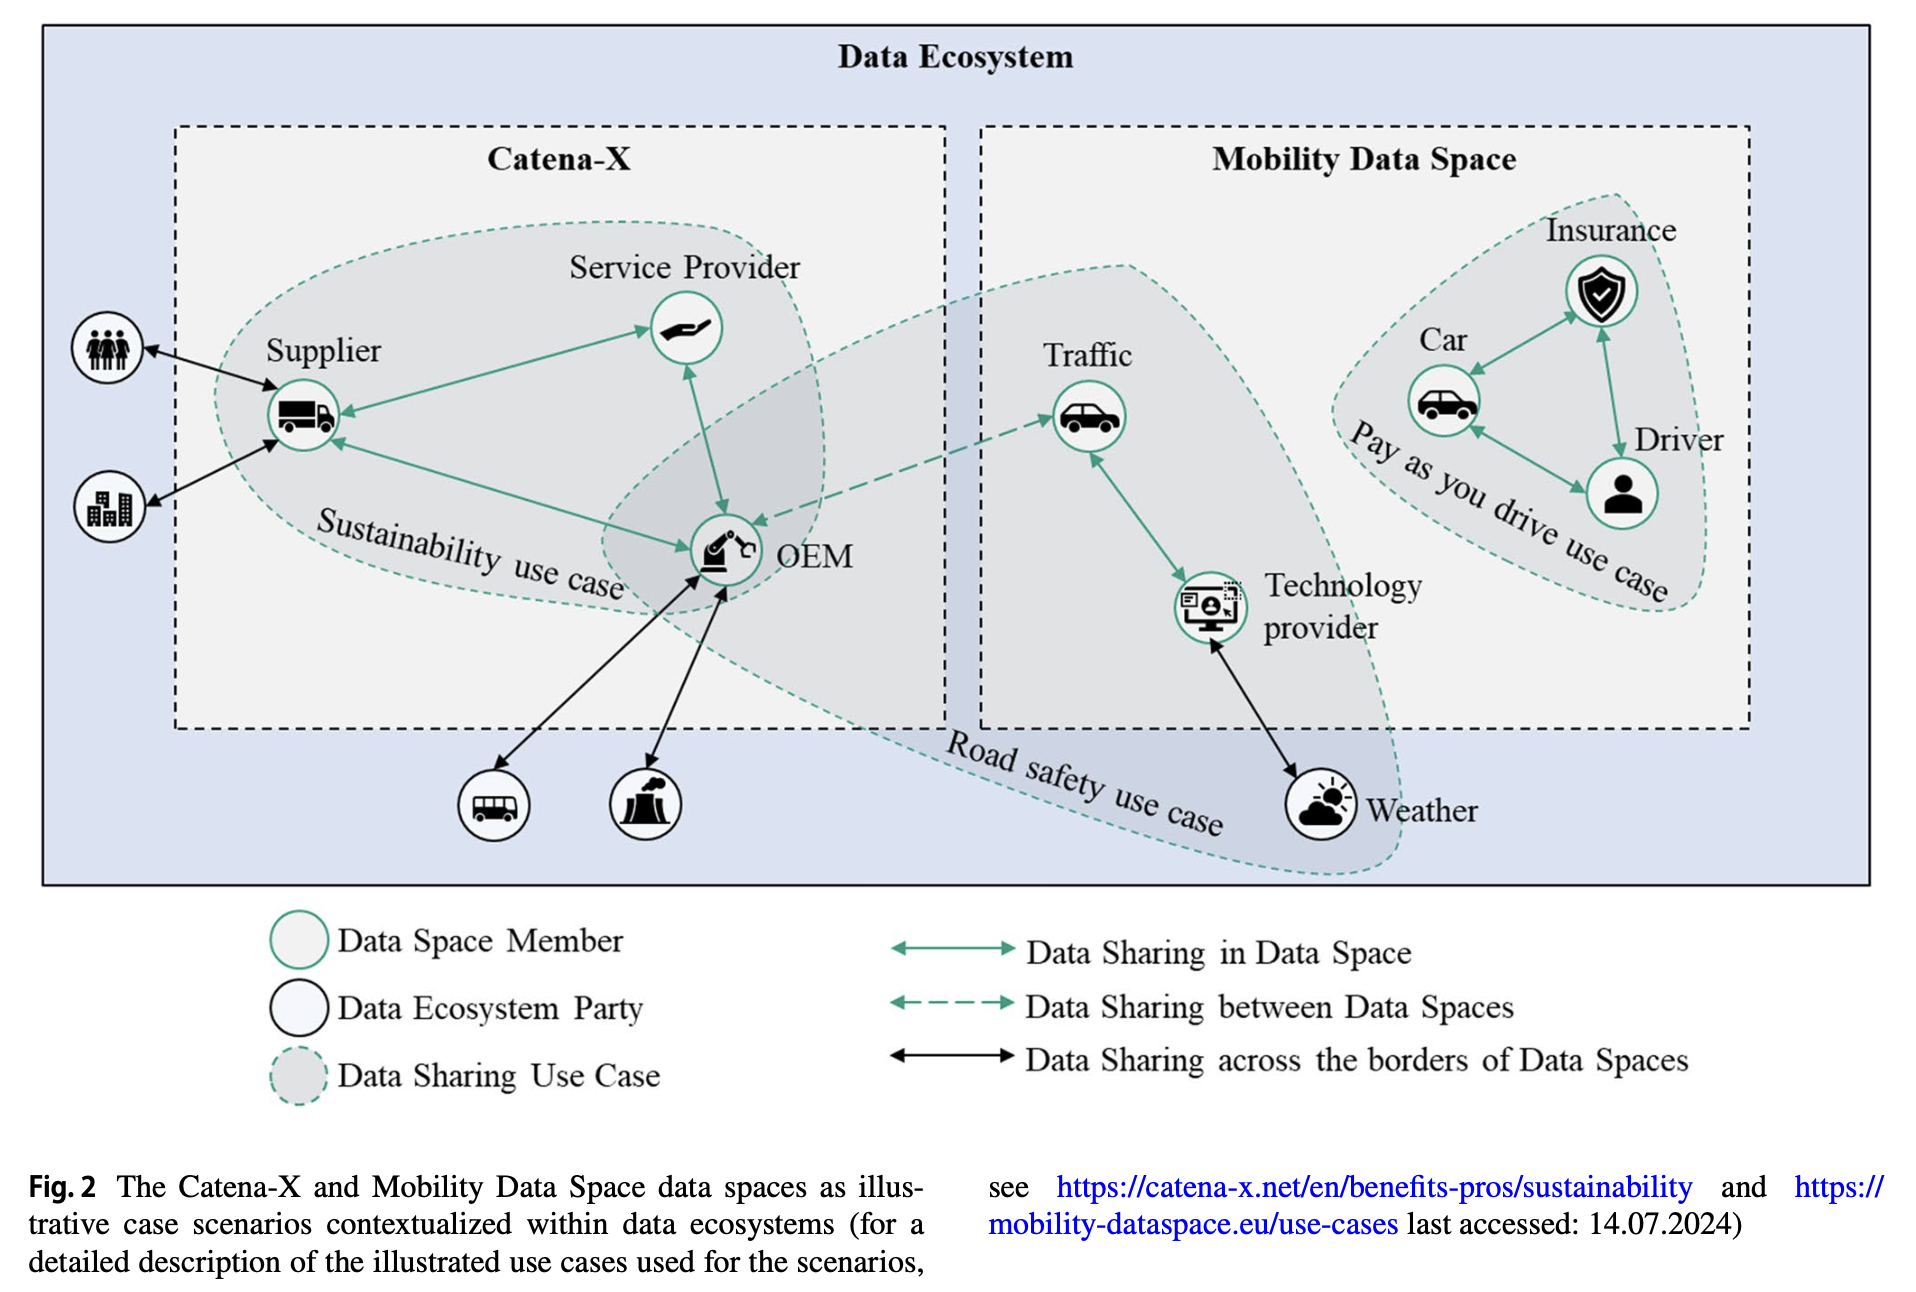
\includegraphics[width=\textwidth]{./assets/moller_data_ecosystem.png}
%     \caption{Data Ecosystem mit Data Space Member und Data Ecosystem Parties am Beispiel von Catena-X und Mobility Data Space~\cite{mollerIndustrialDataEcosystems2024}}
%     \label{fig:data-ecosystem}
%     % TODO: Bild ersetzen, Zusammenführung mit versch. Szenarien für DE
% \end{figure}
